\documentclass{article}

\usepackage[utf8]{inputenc}
\usepackage[T1]{fontenc}
\usepackage[francais]{babel}
\usepackage{titling}
\setlength{\droptitle}{-3cm}
\usepackage{graphicx}
\usepackage{underscore}
\usepackage{hyperref} 
\usepackage{wrapfig}

\title{Interprétation des résultats}
\author{CAROT Axel, ARISOY Ivan Can}
\date{\today}

\begin{document}
\maketitle

%%%%%%%%%%%%%%%%%%%%%%%%%%%%%%%%%%%%%%%%%%%%%%%%%%%%%%%%%%%%%%%%%%%%%%%%%

\section{Classification}
Nos premiers résultats de classification nous ont montré que, malgré une bonne compréhension de la structure de notre corpus, les performances sur les tests n’étaient pas parfaites. C’est-à-dire qu'avec un jeu de données d'entraînement équilibré en termes de classes, et un préentrainement de classification des textes avec un jeu de données d'entraînement et de validation, nous avons obtenu de bons résultats en termes d’accuracy sur le test. Tandis que notre modèle était plutôt bon pour classer correctement les textes non pertinents, ce qui résultait en un faible rappel. Cette observation est clairement visible dans une matrice de confusion:\\

\begin{figure}[!htbp]
    \centering
    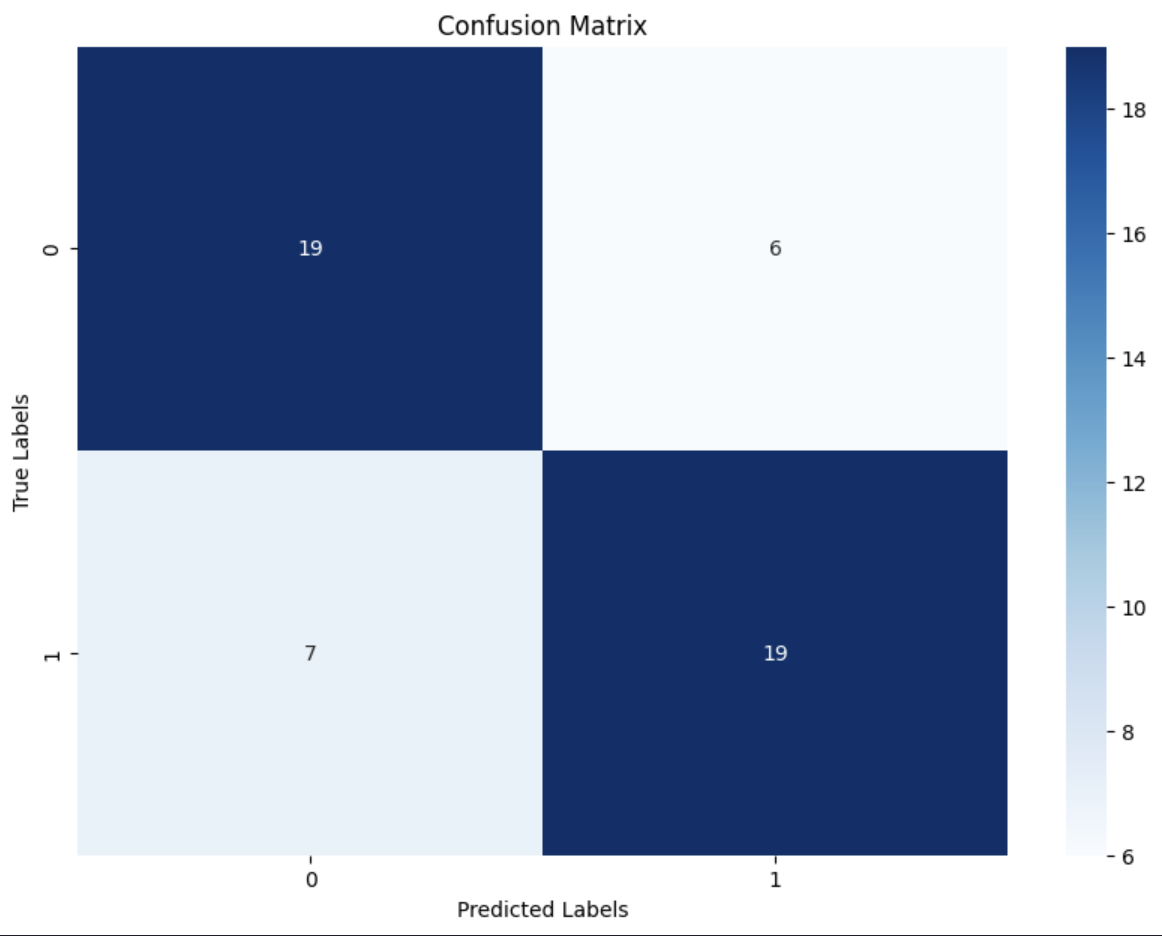
\includegraphics[width=0.55\textwidth]{confusion1.png}
    \caption{Matrice de confusion du premier modèle}
    \label{fig:plots}
\end{figure}

Après avoir discuté avec nos professeurs, un entraînement plus approfondi a été conseillé sous forme de "transfer learning". Une des méthodes courantes pour effectuer cela est le préentraînement par masquage de mots (Masked Language Modeling). L'idée était de faire apprendre à notre modèle les nuances spécifiques de notre corpus afin d'enrichir l'espace de représentation des caractéristiques, puis procéder au preéntraînement de classification.\\

Puisque nous utilisons des pratiques telles que le « shuffle » et ensuite le « stratify » pour maintenir le ratio des labels dans les jeux de données, nous utilisons également le même random state pour conserver l'état de notre jeu de données pour comparer les résultats sans préentraînement avec ceux obtenus après le masquage.

\subsection{MLM}

\begin{figure}[!htbp]
    \centering
    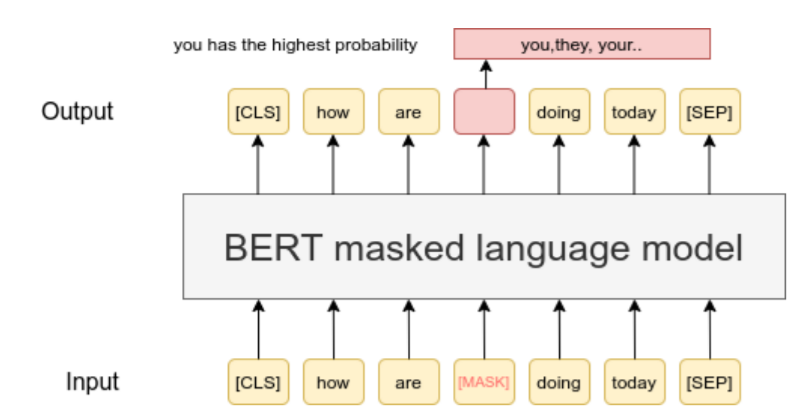
\includegraphics[width=0.6\textwidth]{MLM-2.png}
    \caption{- www.sbert.net}
    \label{fig:plots}
\end{figure}


Habituellement, le préentraînement avec masquage consiste à masquer 15\% des tokens d’un texte. Ensuite, le modèle essaie de prédire les mots les plus probables derrière le masque en se basant sur les embeddings. Cela permet de développer une compréhension profonde du contexte linguistique et des relations entre les mots dans le corpus. Pour cette phase complémentaire, nous avons repris notre jeu de données d'entraînement et une première tentative a été effectuée.\\

\subsection{Stratégie de masquage}
Tout d'abord, nous avons remarqué que nous masquions souvent des mots peu significatifs, tels que les stop words. Pour éviter cela et mieux apprendre la structure de nos textes pertinents et non pertinents, nous avons défini une stratégie de masquage plus ciblée sur les mots significatifs et sur les mots du lexique de notre corpus qui nous avaient été fournis au début de notre projet (LEXG, LEXA, LEXC).\\

\begin{itemize}
    \item Premièrement, nous avons défini une liste d'exclusion comprenant des mots de liaison et des caractères spéciaux.
    \item Ensuite, nous avons défini une liste de mots prioritaires à masquer, sélectionnés à partir du lexique fourni.
\end{itemize}
\vspace{10pt}

Pour le masquage, nous maintenons le ratio de 15\% de tokens à masquer. Ensuite, nous fixons une limite de 30\% parmi ces 15\% pour masquer les mots prioritaires issus du lexique, à condition qu'ils soient présents dans le texte.\\

Ce choix a été fait pour éviter un surapprentissage potentiel tout en ne masquant que  30\% au maximum des ces tokens du lexique. La création d'une liste d'exclusion était plus facile à implémenter que de cibler des mots de liaison par un autre outil ou une technique de TALN.

\subsection{Resultats de MLM}

\begin{figure}[!htbp]
    \centering
    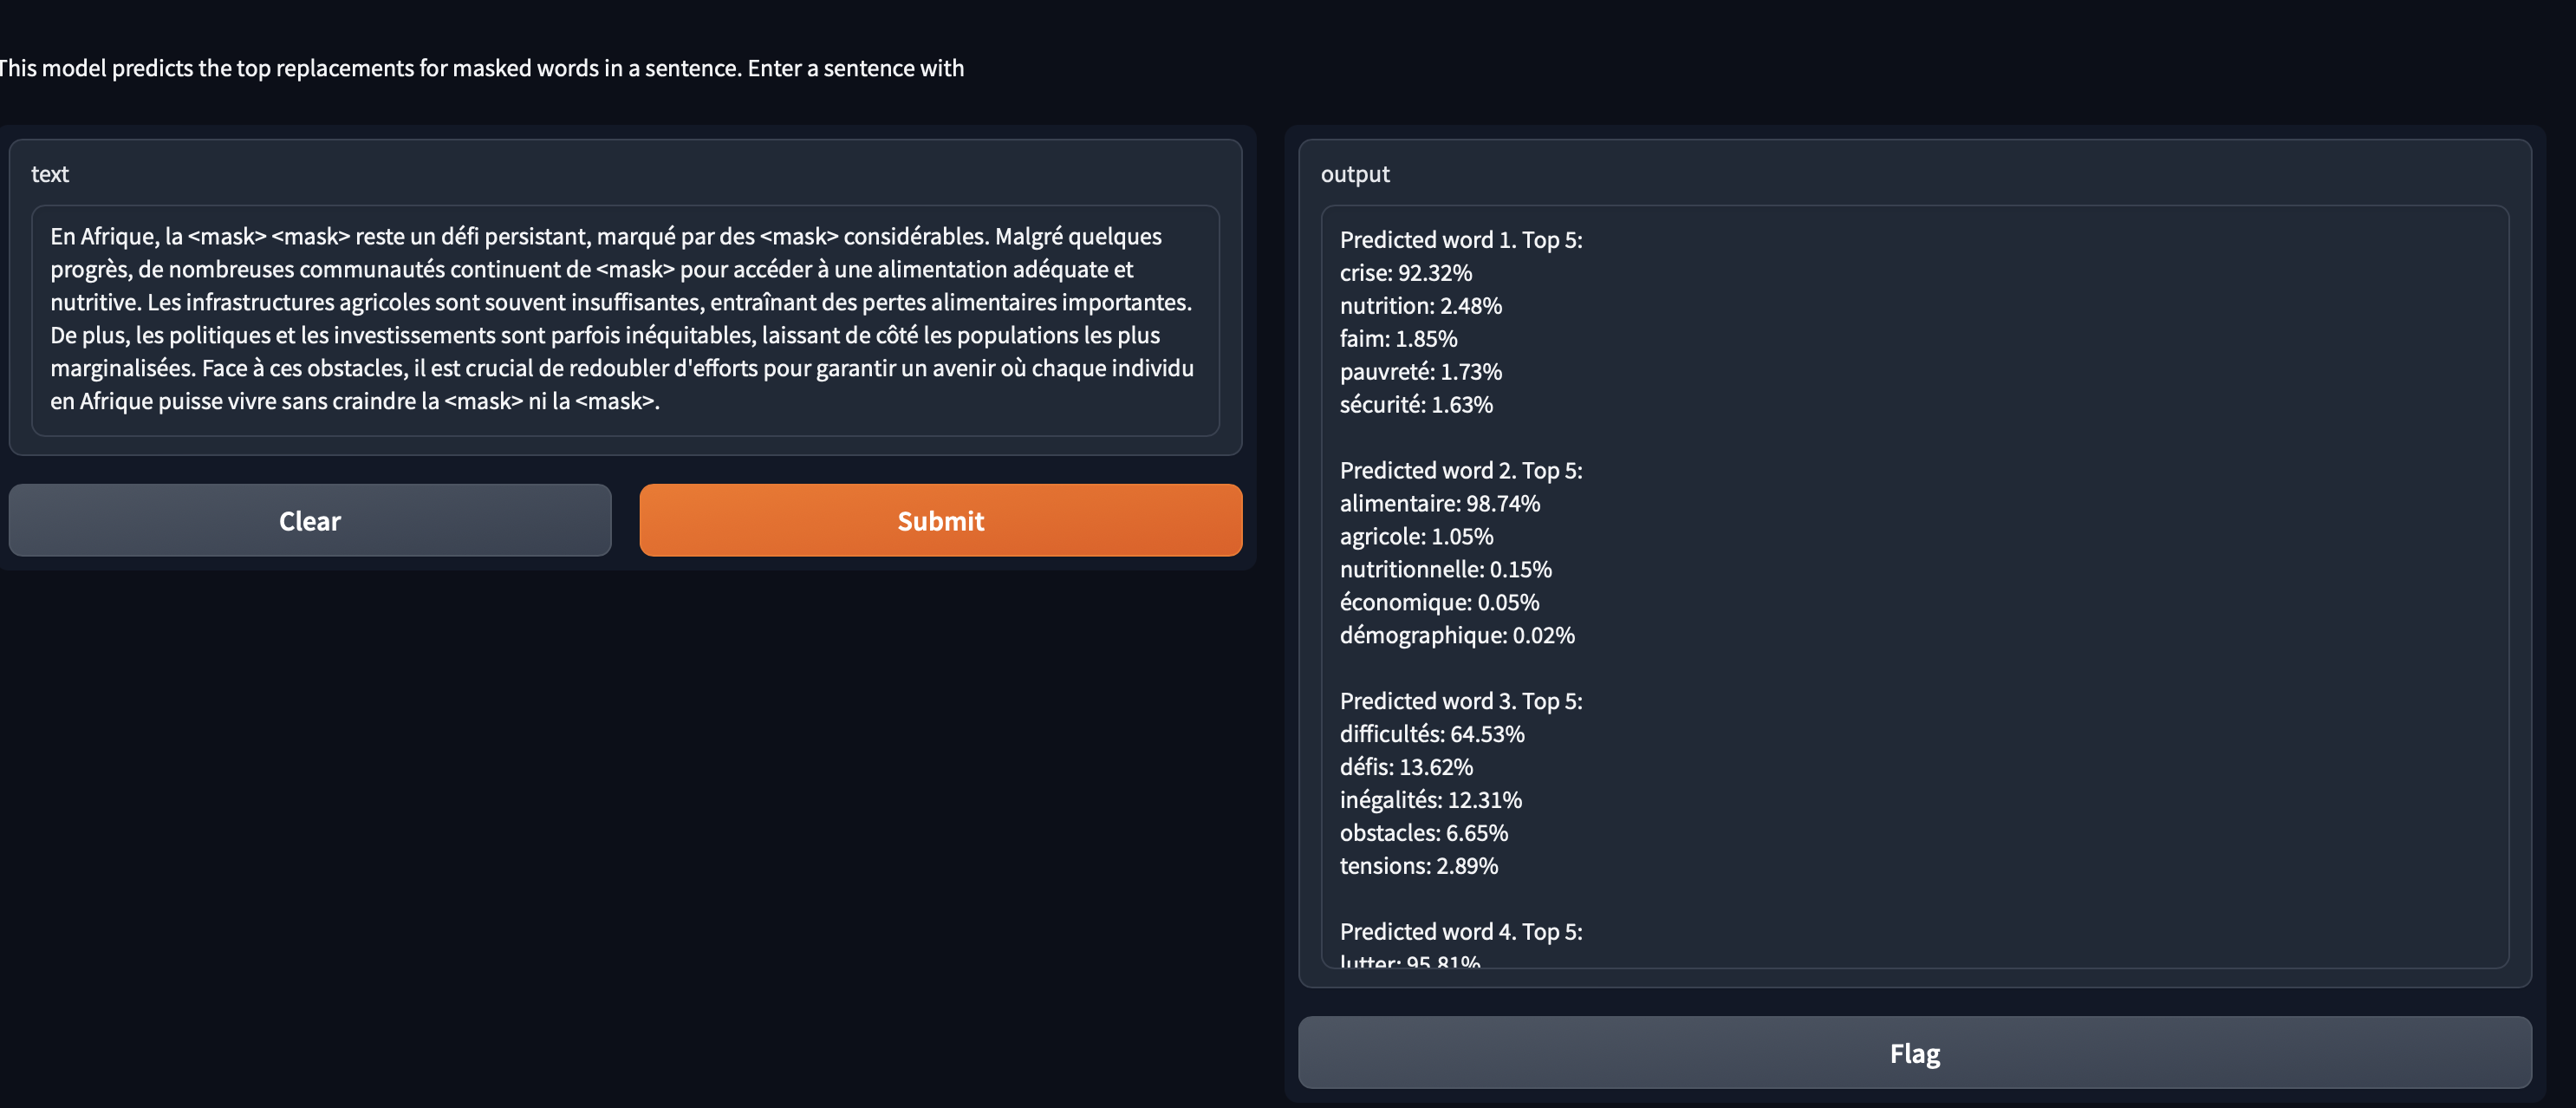
\includegraphics[width=0.9\textwidth]{mlm.png}
    \caption{Visualisation des résultats}
    \label{fig:plots}
\end{figure}

Notre objectif était de vérifier comment notre modèle s’est adapté et s'il a enrichi la représentation de l'espace des caractéristiques, sans se focaliser uniquement sur l'accuracy des mots prédits. Pour tester cela, nous avons comparé notre modèle préentrainé à un modèle \textit{'camemBERT for masked LM'} sans préentrainement sur notre corpus. Ensuite, nous avons choisi un texte aléatoire traitant directement de l'insécurité alimentaire en Afrique, et nous avons masqué plusieurs mots-clés, parfois deux tokens d'affilée, pour voir comment le modèle allait reconstruire la phrase.\\



Nous avons observé que notre modèle préentrainé prédisait les mots de manière précise et conforme au contexte spécifique de la sécurité alimentaire, tandis que le modèle sans préentraînement optait souvent pour des termes plus généraux, typiques des crises, mais moins pertinents pour notre sujet. Cette différence illustre comment les résultats du modèle sans préentraînement tendaient à dévier de nos objectifs spécifiques. Voici quelques exemples où nous comparons le mot le plus probable prédit par chaque modèle :\\



\textbf{Les mots masqués}: \texttt{sécurité}, \texttt{alimentaire}, \texttt{faim}, \texttt{malnutrition}.\\

\begin{displayquote}
``En Afrique, la \texttt{\textlangle{}mask\textrangle{}} \texttt{\textlangle{}mask\textrangle{}} reste un défi persistant (...) Face à ces obstacles, il est crucial de redoubler d'efforts pour garantir un avenir où chaque individu en Afrique puisse vivre sans craindre la \texttt{\textlangle{}mask\textrangle{}} ni la \texttt{\textlangle{}mask\textrangle{}}.''
\end{displayquote}

\begin{tabular}{|l|l|l|l|l|}
\hline
\textbf{Modèle} & \textbf{Mot 1} & \textbf{Mot 2} & \textbf{Mot 3} & \textbf{Mot 4} \\ \hline
Avec préentraînement & \texttt{crise} & \texttt{alimentaire} & \texttt{faim} & \texttt{famine} \\ \hline
Sans préentraînement & \texttt{crise} & \texttt{économique} & \texttt{pauvreté} & \texttt{pauvreté} \\ \hline
\end{tabular}


\subsection{Préentrainement de Classification après le MLM}

Nous avons ensuite abordé le préentraînement classique pour la classification avec 334 textes labellisés. Nous avons opté pour un \textit{learning rate} de $3 \times 10^{-5}$, un \textit{batch size} de 16, AdamW comme optimiseur, et nous avons pris le meilleur modèle en termes d'accuracy après 10 épisodes. La division de notre jeu de données s'est faite en ensembles d'entraînement, de validation et de test. Ces hyperparamètres ont été choisis après quatre essais sur le jeu de validation afin de minimiser l'introduction de biais dans notre modèle. Néanmoins, nous envisagions d'utiliser une approche plus avancée pour la sélection des modèles et des hyperparamètres, notamment la \textit{Nested Cross-validation}. Cependant, cette approche étant assez longue et coûteuse, nous n'avons pas de résultats concrets pour le moment.\\

En ce qui concerne la tokenisation, de nombreux textes comportent plus de 512 tokens. Afin d'éviter une perte d'information, nous avons choisi de tokeniser les 256 premiers et les 256 derniers tokens.

\section*{Résultats de Classification}

Nous avons observé de bons résultats sur le jeu de données de test. Malheureusement, nous nous sommes trompés dans la labellisation de certains textes. Après vérification, nous avons corrigé les annotations erronées.

\begin{figure}[!htbp]
    \centering
    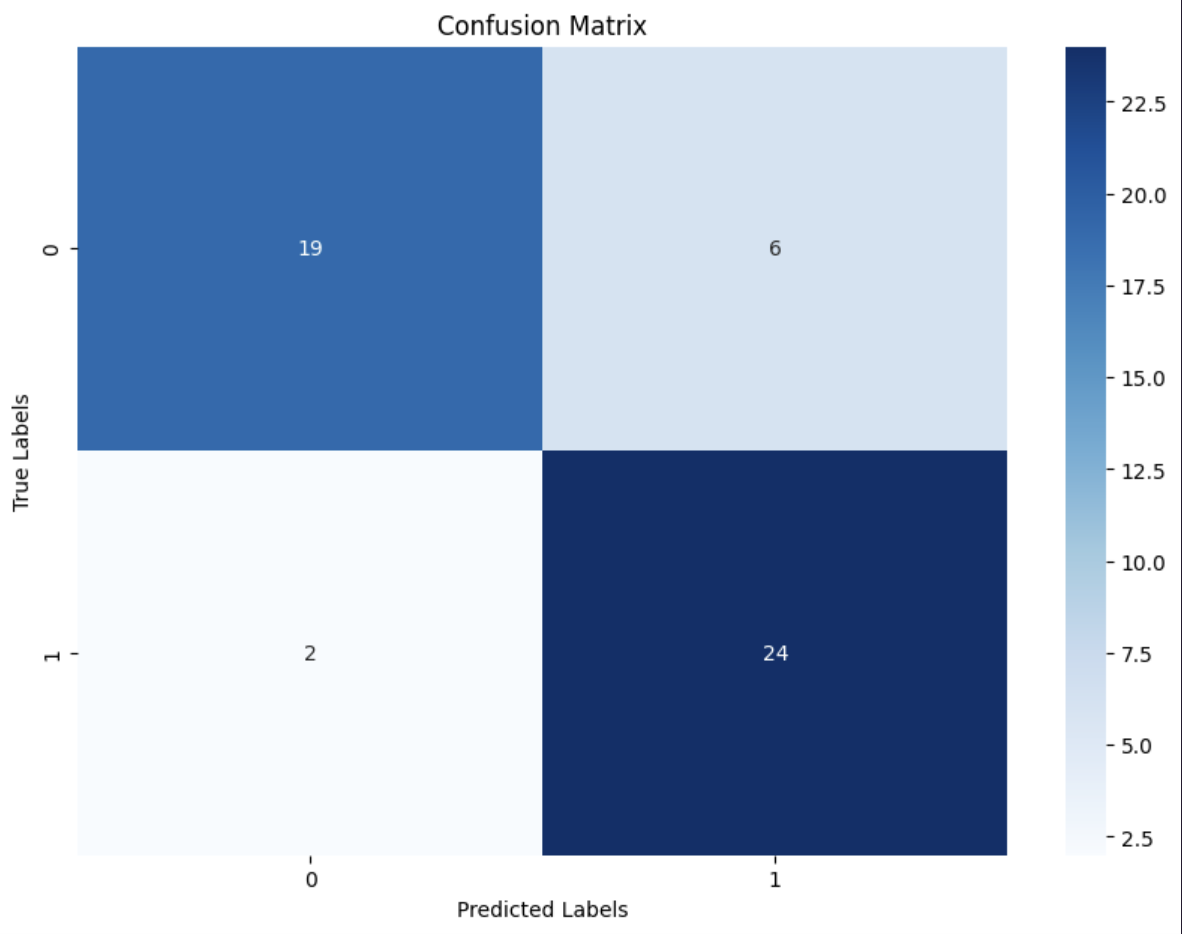
\includegraphics[width=0.6\textwidth]{confusion2.png}
    \caption{Matrice de confusion du dernier modèle}
    \label{fig:plots}
\end{figure}

Nous avons ensuite utilisé le dernier modèle pour prédire les labels de 9410 textes du corpus. Auparavant, les étiquettes de ce corpus avaient déjà été prédites avec un premier modèle sans préentraînement avec le MLM. Ainsi, nous avons utilisé les premières prédictions pour les comparer aux nouvelles.\\

Notre premier modèle a identifié seulement 356 textes pertinents dans le corpus, tandis que le deuxième en a pu identifier 999. C'est un résultat assez satisfaisant d'avoir trouvé davantage de textes pertinents qu'auparavant. Toutefois, ces résultats, ainsi que le modèle, ont encore une marge d'amélioration.

%%%%%%%%%%%%%%%%%%%%%%%%%%%%%%%%%%%%%%%%%%%%%%%%%%%%%%%%%%%%%%%%%%%%%%%%%

\section{Analyses des sentiment des articles pertinents}

Nous avons opté pour deux méthodologies distinctes d'analyse des sentiments. La première s'appuie sur la bibliothèque Python TextBlob, qui permet la détection de la polarité et de la subjectivité dans les textes. Ensuite, nous utilisons BERT, un modèle de pré-entraînement qui est beaucoup plus avancée et complexe que celle de TextBlob. \\

Notre but est d'observer les écarts entre les résultats produits par ces deux approches. On s'attend à ce que l'analyse de sentiment à l'aide de BERT révèle une compréhension plus nuancée et contextuelle des textes, grâce à sa capacité à saisir les subtilités, alors que TextBlob pourrait donner des résultats plus rapides et plus généralistes, mais moins précis dans l'interprétation des sentiments complexes ou implicites.

\subsection{Analyses de sentiment avec TextBlob}
Nous utilisons la polarité généré par textblob pour classé les textes en trois catégories de sentiments : Positif, Neutre, Négatif. Pour cela, nous avons en premier lieux observer la distribution de la polarité pour déterminer les seuils appropriés à cette classification.

\begin{figure}[!htbp]
    \centering
    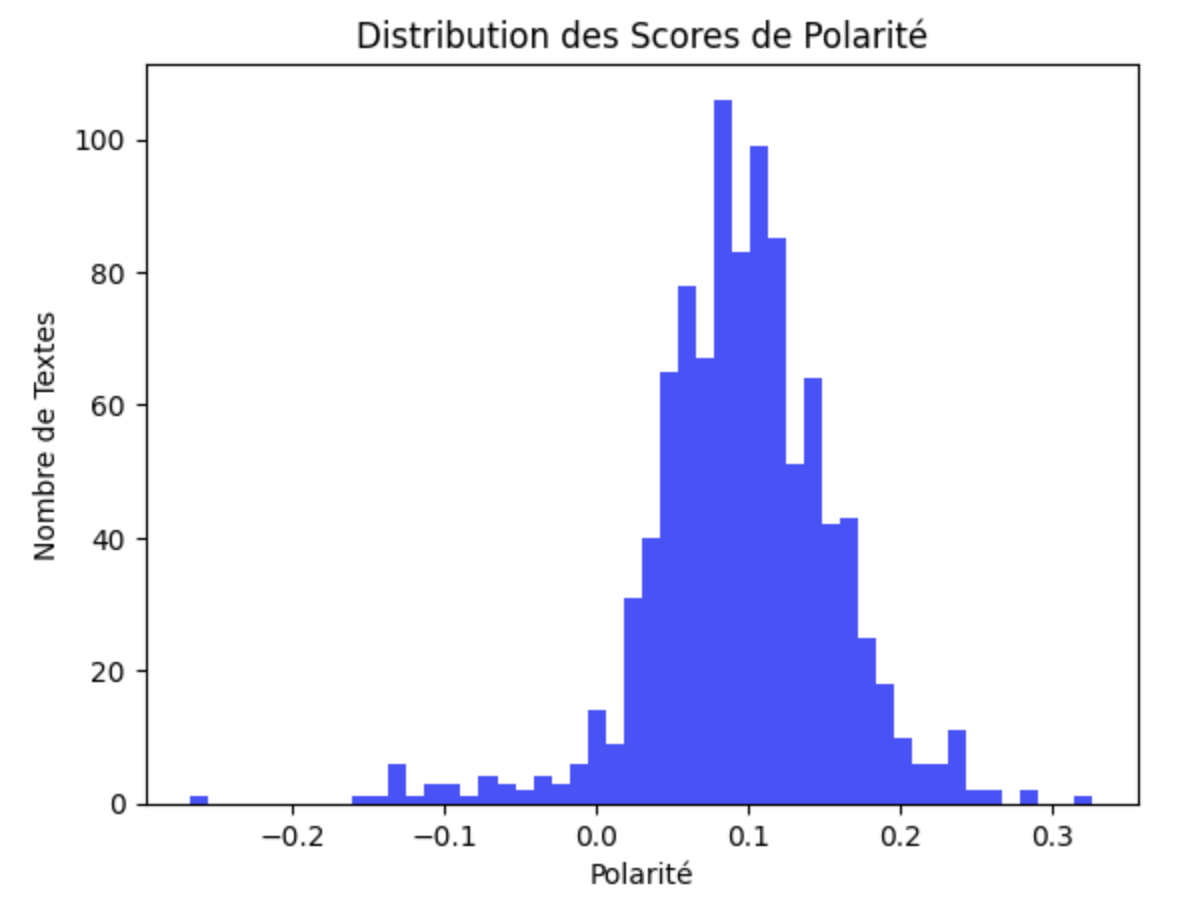
\includegraphics[width=0.4\textwidth]{polarite_distrib.png}
    \caption{Distribution des Scores de Polarité}
    \label{fig:plots}
\end{figure}

Nous observons que la majorité de nos textes présentent une polarité supérieure à zéro, ce qui indiquerait a priori une tendance vers des sentiments positifs. Toutefois, une lecture de plusieurs textes au sein des différentes catégories de sentiments révèle que notre corpus est composé essentiellement de textes négatifs. Par conséquent, nous avons ajusté nos seuils de polarité pour la classification des sentiments afin de mieux correspondre au contexte spécifique de notre ensemble de données. Nous avons établi les seuils suivants :
\\
\begin{itemize}
    \item Polarité > 0.15 : Positif
    \item 0.13 > Polarité > 0.15 : Neutre
    \item Polarité < 0.13 : Négatif
\end{itemize}

\begin{figure}[!htbp]
    \centering
    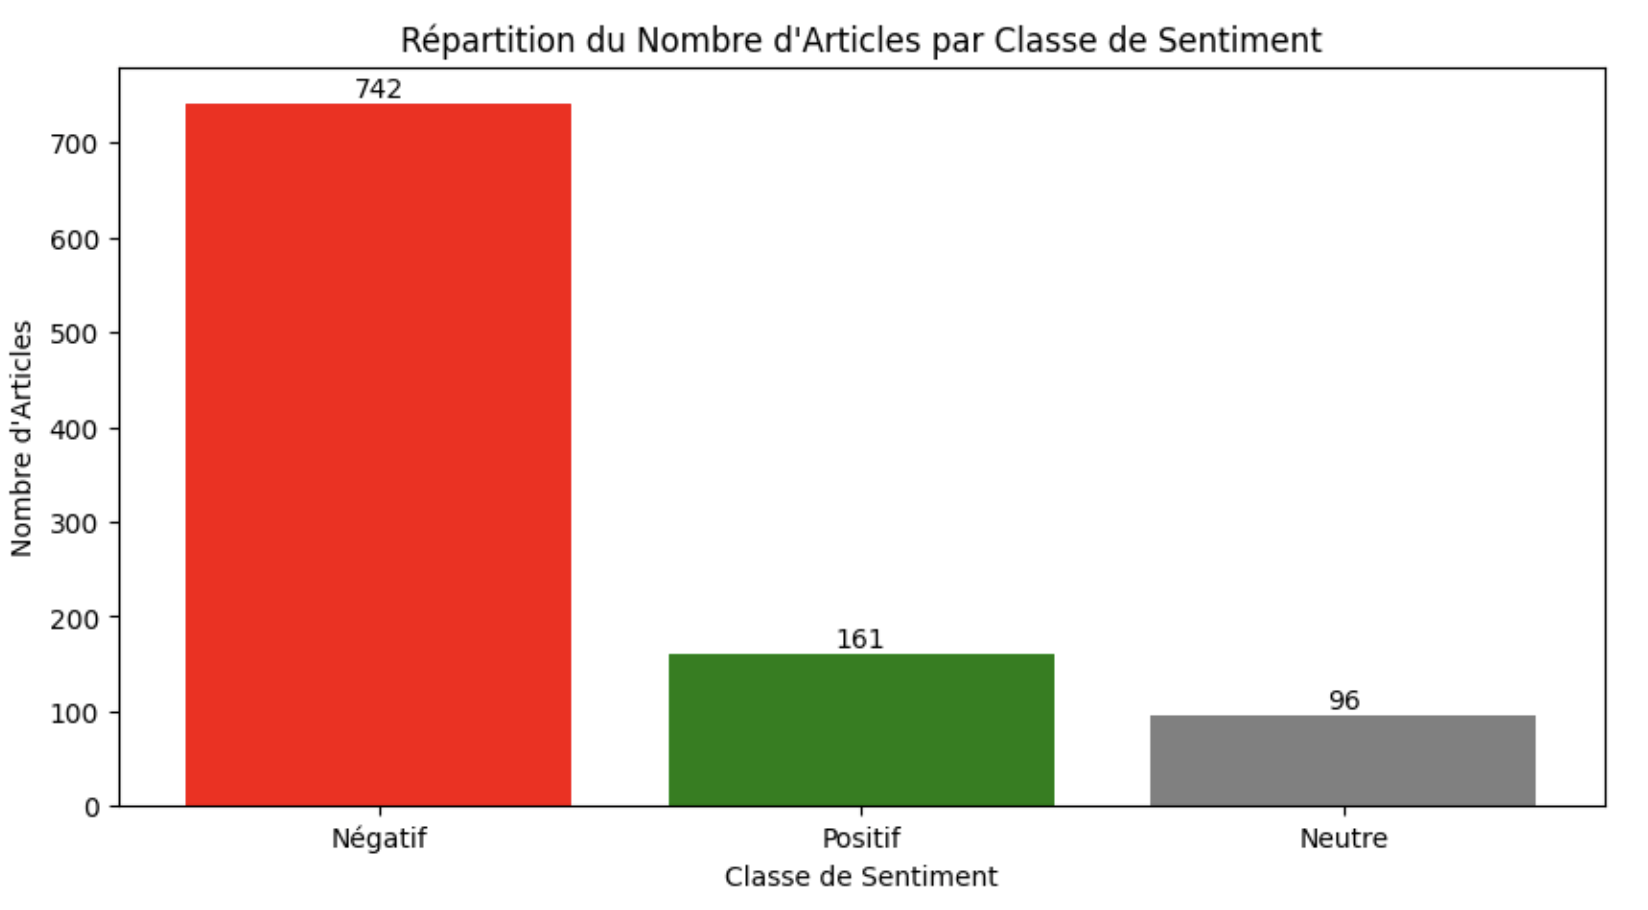
\includegraphics[width=0.5\textwidth]{repartition_textBlob.png}
    \caption{Répartition des classes de sentiment avec TextBlob}
    \label{fig:plots}
\end{figure}

\subsection{Analyses de sentiment avec BERT}
Nous avons utilisé BERT pour classer nos textes en 5 classes de sentiment allant de 0 pour les textes très négatifs à 4 pour les textes très positifs. BERT génère également un score de confiance relatif à la classe attribuée.

\begin{figure}[!htbp]
    \centering
    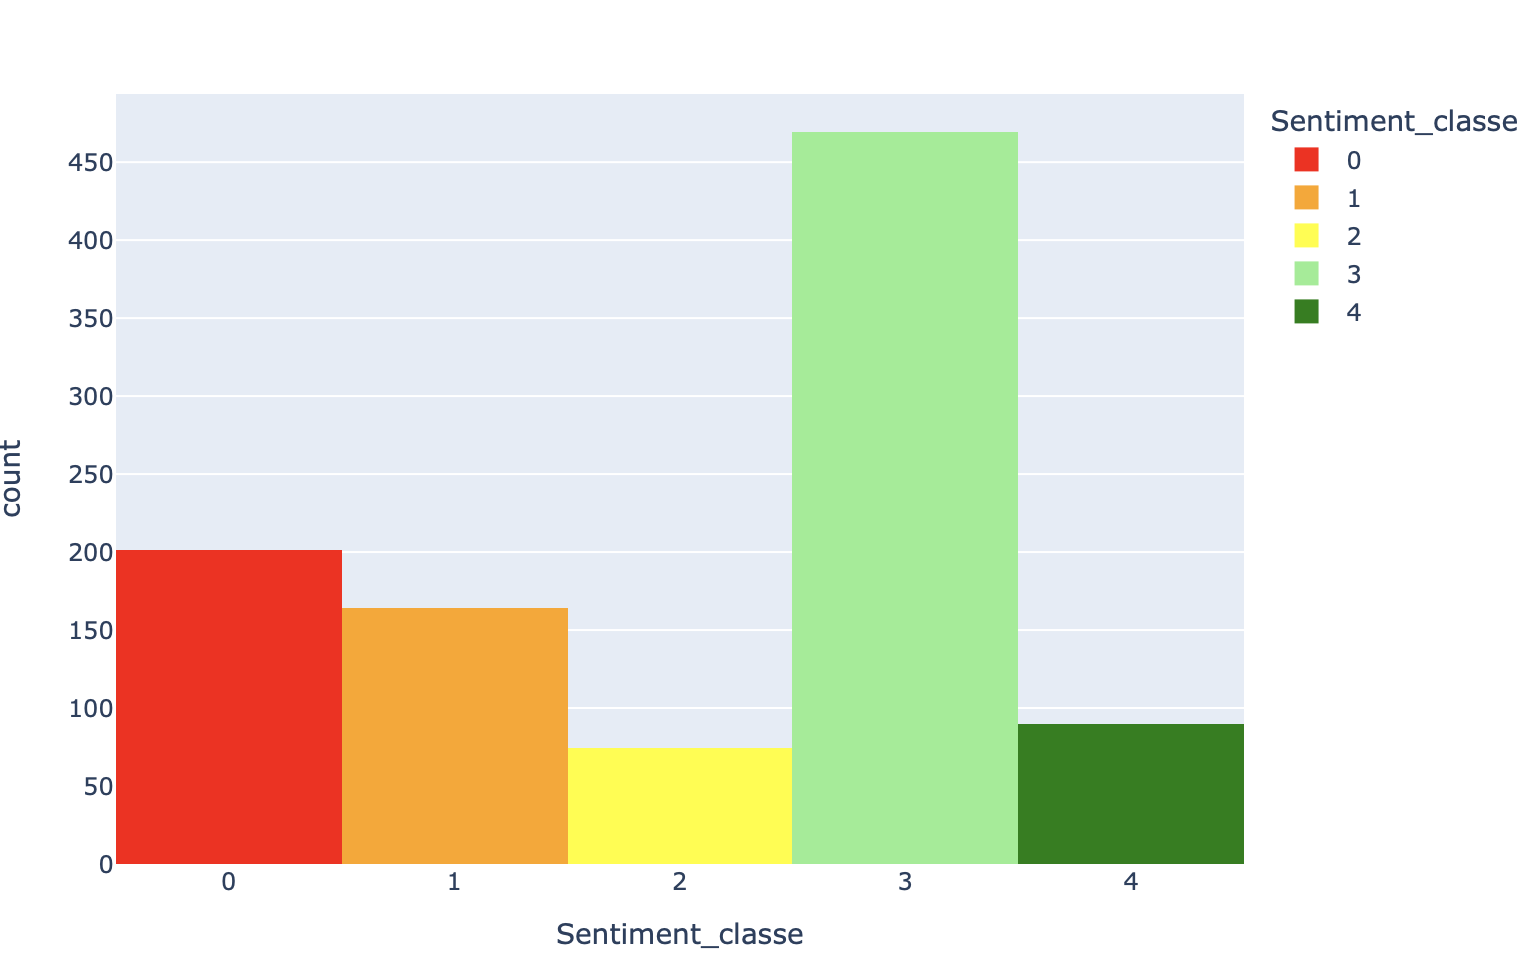
\includegraphics[width=0.5\textwidth]{repartition_bert.png}
    \caption{Répartition des classes de sentiment avec BERT}
    \label{fig:plots}
\end{figure}
\vspace{-0.4cm}

\subsection{Comparaison des deux analyses de sentiment}
La comparaison des analyses de sentiment réalisées avec TextBlob et BERT montrent des différences dans la classification des émotions. Avec TextBlob, nous avons une tendance marquée vers des sentiments positifs, comme le montre la distribution de la polarité. Cela peut être dû à sa simplicité car il se base sur des mots clés pour déterminer la polarité, et peut ne pas saisir le contexte qui pourrait être présent dans les textes.\\

En revanche, BERT, qui analyse le contexte de manière plus approfondie, répartit les sentiments de façon plus uniforme sur cinq classes. Cependant, contrairement à nos attentes et malgré le contexte négatif des textes, les résultats indiquent aussi une prédominance de sentiments positifs, particulièrement dans la catégorie 3. Cela suggère que la classification des sentiments peut varier en fonction des modèles et des méthodes utilisées, et que l'ajustement des seuils et des paramètres pourrait être nécessaire pour aligner les résultats avec le contexte de notre corpus.

\begin{figure}[!htbp]
    \centering
    \includegraphics[width=0.5\textwidth]{corrélation.png}
    \caption{Matrice de corrélation}
    \label{fig:plots}
\end{figure}

L'analyse de la matrice valide la corrélation entre SentimentBlob et Polarity ce qui est cohérent étant donné que le sentiment (SentimentBlob) est déterminé à partir de la polarité. La faible corrélation entre les autres variables suggère qu'elles reflètent divers aspects sentimentales des données. ConfidenceMlm, qui mesure la confiance liée à la classification de la pertinence des articles, n'est pas nécessairement liée à la polarité ou la subjectivité des textes. Par exemple, un texte peut être clairement classé comme pertinent avec une haute confiance, mais cela ne dit rien sur le degré de sa subjectivité ou de sa polarité. Les non corrélations entre les variables Subjectivity, SentimentBERT et SentimentBlob reflètent la complexité de l'analyse sentimentale quand elle est réalisé avec différentes techniques. 

\section{Clustering des textes pertinents avec BERT}

Notre objectif pour le clustering de nos textes pertinents est de trouver des groupes de documents qui partagent des thématiques et des sentiments similaires, afin de pouvoir résumer efficacement les tendances dominantes et les opinions au sein du corpus analysé. \\

Nous espérons observer que les clusters basés sur les embeddings de BERT 
valident les groupes d'articles trouvés grâce à nos analyse de sentiments. \\

Pour cela, nous effectuons le clustering uniquement à l'aide des textes de nos articles. Avec BERT, nous tokenisons les textes. Ensuite, nous effectuons l'extraction de caractéristiques. Grâce aux tokens, BERT génère un ensemble de vecteurs d'embeddings pour chaque texte. Ces vecteurs capturent les nuances sémantiques et contextuelles des textes et servent de base pour le clustering, permettant ainsi de regrouper les textes selon leur similarité. \\

\begin{figure}[!htbp]
    \centering
    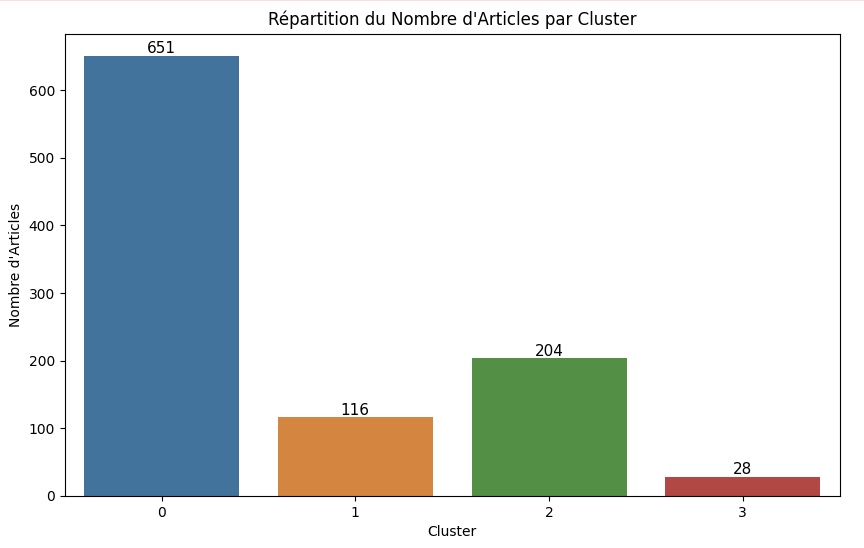
\includegraphics[width=0.6\textwidth]{repartition_cluster_bert.png}
    \caption{Répartition du Nombre d'Articles par Cluster}
    \label{fig:plots}
\end{figure}

Pour interpréter nos cluster, nous commençons par visualiser les mots plus fréquents selon leur fréquence d'apparition dans les textes de chaque cluster ainsi que les articles les plus proches des centroîdes qui sont déterminés en fonction de leur distance vectorielle par rapport au centroïde dans l'espace des caractéristiques. Cette analyse ne révèle pas de thématiques évidentes au sein de nos groupes d'articles. \\

Pour approfondir l'interprétation de nos clusters, nous envisageons d'appliquer un topic modeling ainsi qu'un TF-IDF et d'utiliser la bibliothèque Python Yake. Le topic modeling via LDA, permet d'identifier des thèmes dans les textes, facilitant la compréhension des sujets prédominants et de leur distribution au sein des clusters. Yake sert à extraire automatiquement des mots-clés basés sur leur pertinence statistique dans un document isolé, aidant à identifier rapidement les termes clés qui caractérisent chaque cluster. En complément de Yake, TF-IDF permettrai d'évaluer l'importance d'un mot en tenant compte de sa fréquence dans un document par rapport à sa fréquence dans l'ensemble du corpus. \\

Pour continuer notre analyse des clusters, nous explorons les variables produites par nos analyses de sentiments, suite à l'absence de thématiques évidentes dans l'analyse textuelle initiale. Le but de cette analyse basée sur les variables de sentiments est d'identifier des indicateurs pour différencier les clusters. Pour cela, nous utilisons une visualisation interactive réalisée avec la bibliothèque Python Plotly, qui nous permet d'explorer les sentiments qui caractérisent chaque cluster. \\

\begin{figure}[h]
    \centering
    \begin{minipage}{.5\textwidth}
        \centering
        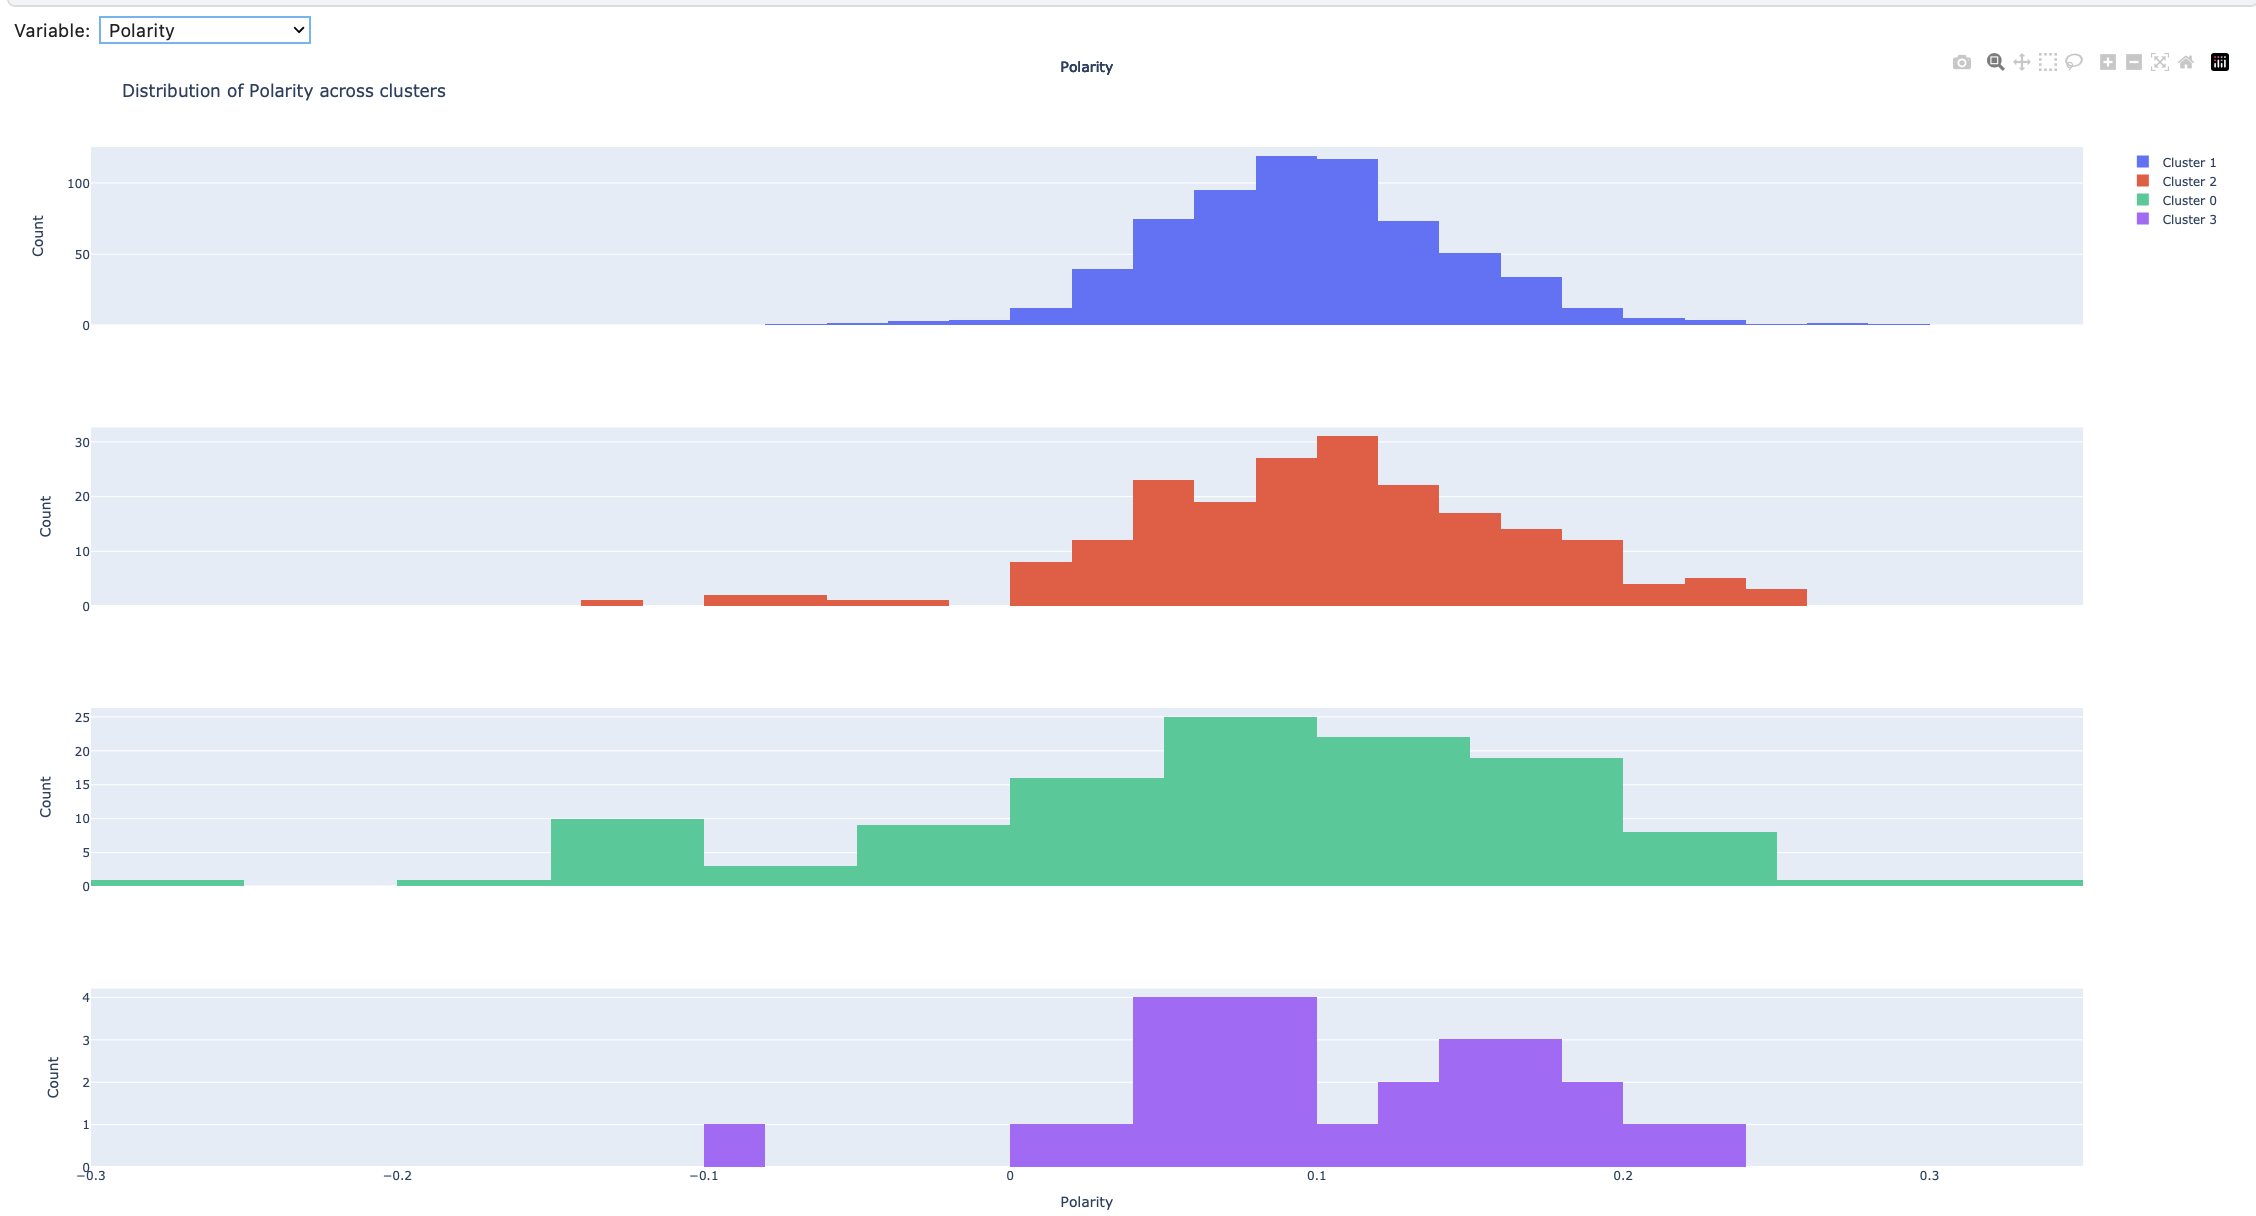
\includegraphics[width=0.9\linewidth]{polarity.png}
        \label{fig:Distribution de la polarité par cluster}
    \end{minipage}%
    \begin{minipage}{.5\textwidth}
        \centering
        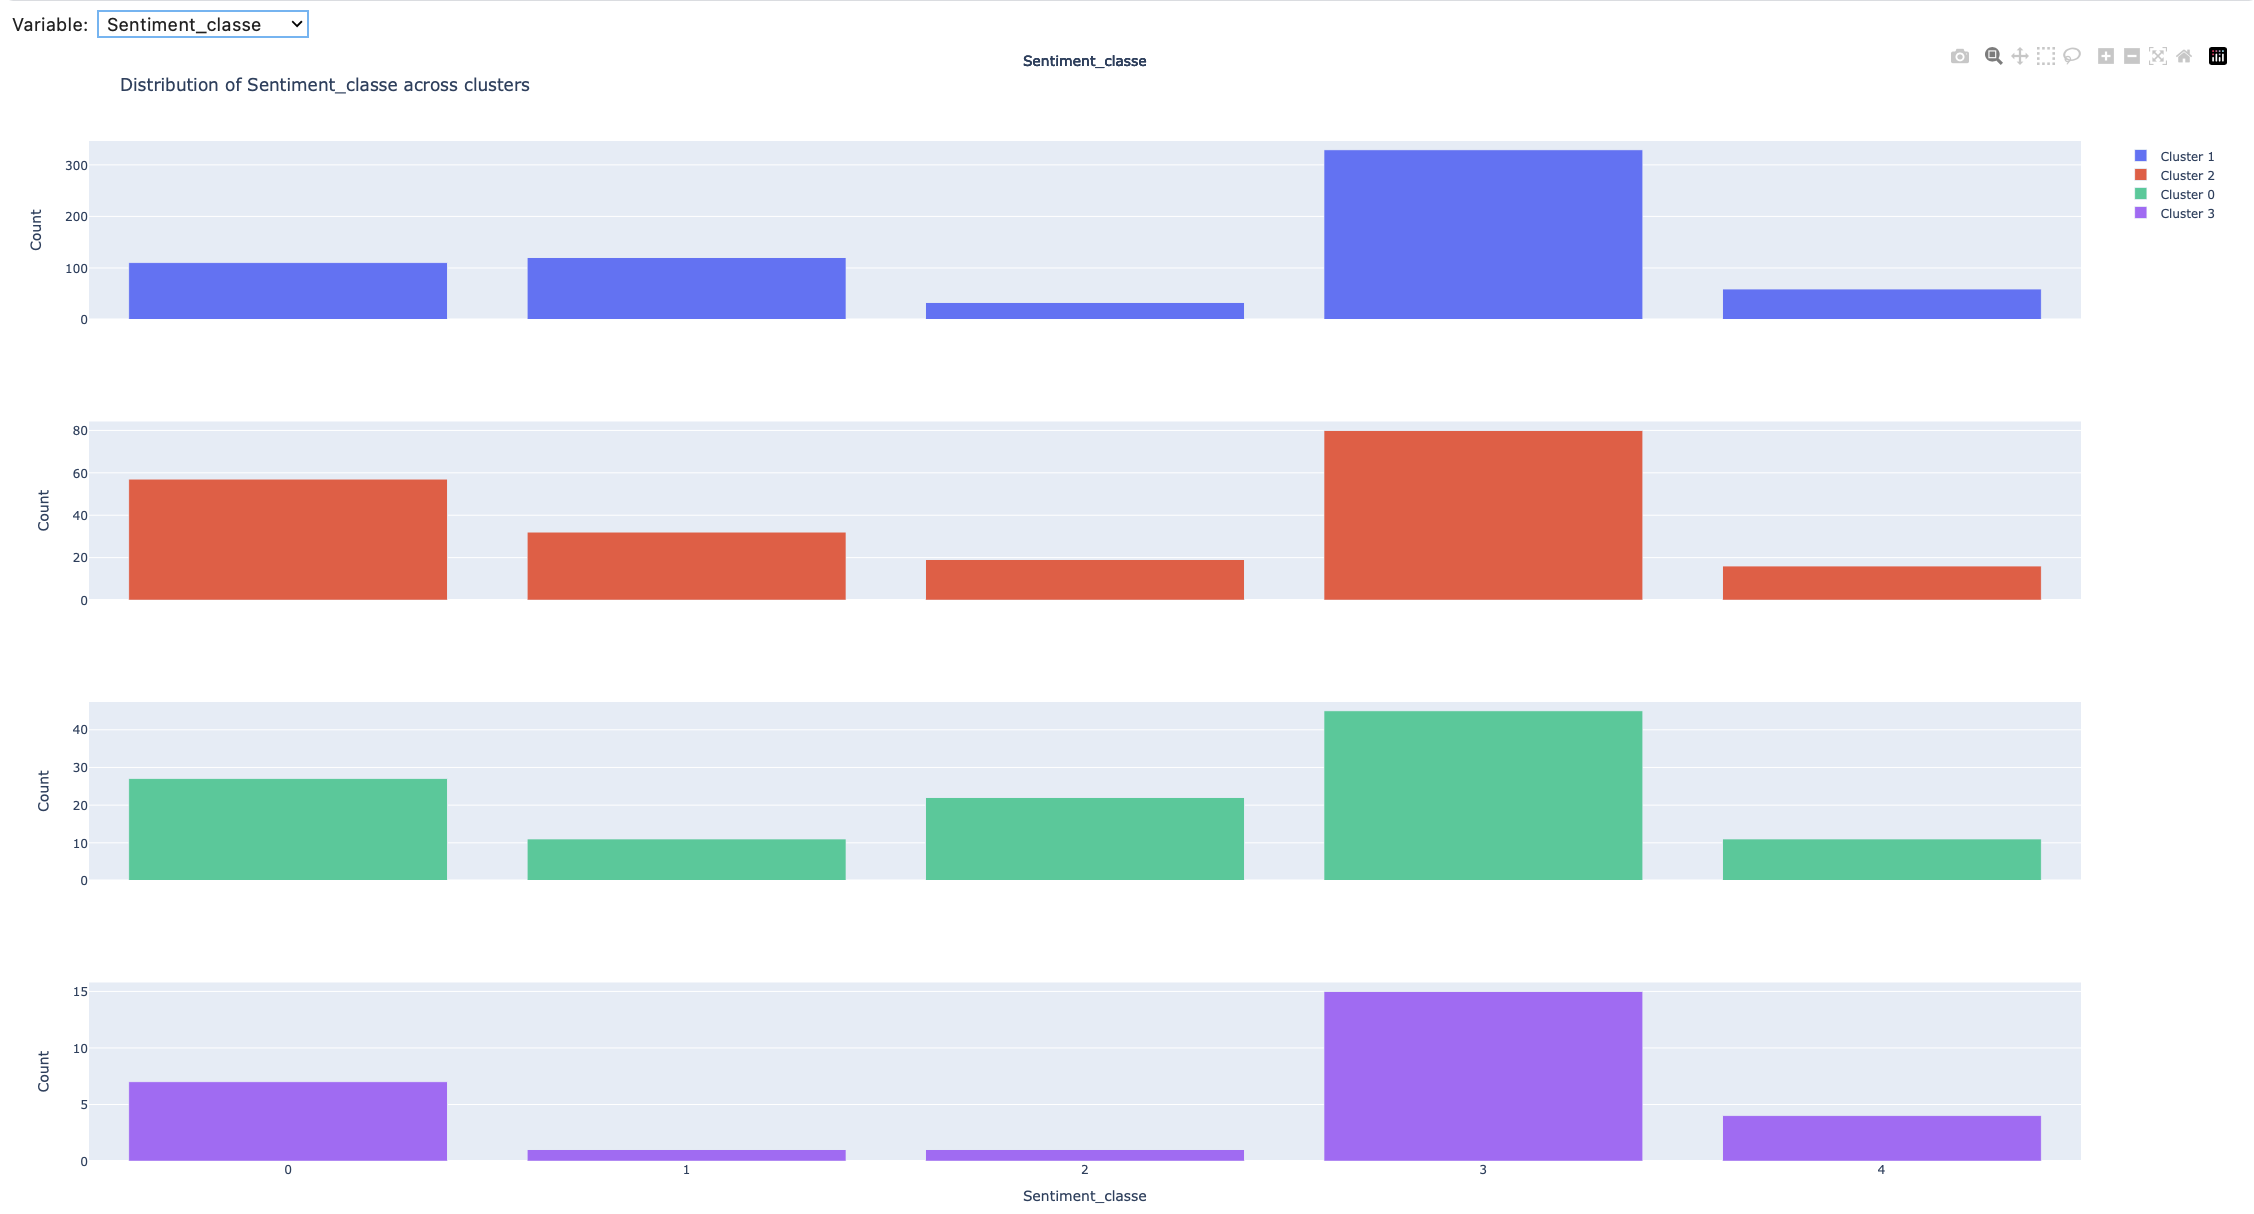
\includegraphics[width=0.9\linewidth]{sentiment_bert.png}
        \label{fig:Distribution des classes de sentiment de BERT par cluster}
    \end{minipage}
    \caption{Distribution de la polarité et des classes de sentiment de BERT par cluster}
\end{figure}
\vspace{3cm}

Nous pouvons constater que les clusters formés à l'aide des embeddings de BERT ne reflètent pas les résultats de notre analyse de sentiment. Cette différence est probablement due au fait que nos clusters intègrent non seulement les thématiques abordées mais aussi des paramètres complexes tels que la cohérence du contexte, la structure syntaxique et les nuances de la langue, qui vont bien au-delà des indicateurs sentimentaux basiques utilisés précédemment. Ces paramètres complexes influencent la formation des clusters de manière différente de nos attentes initiales.

%%%%%%%%%%%%%%%%%%%%%%%%%%%%%%%%%%%%%%%%%%%%%%%%%%%%%%%%%%%%%%%%%%%%%%%%%

\end{document}
